\begin{figure}[ht]
    \centering
    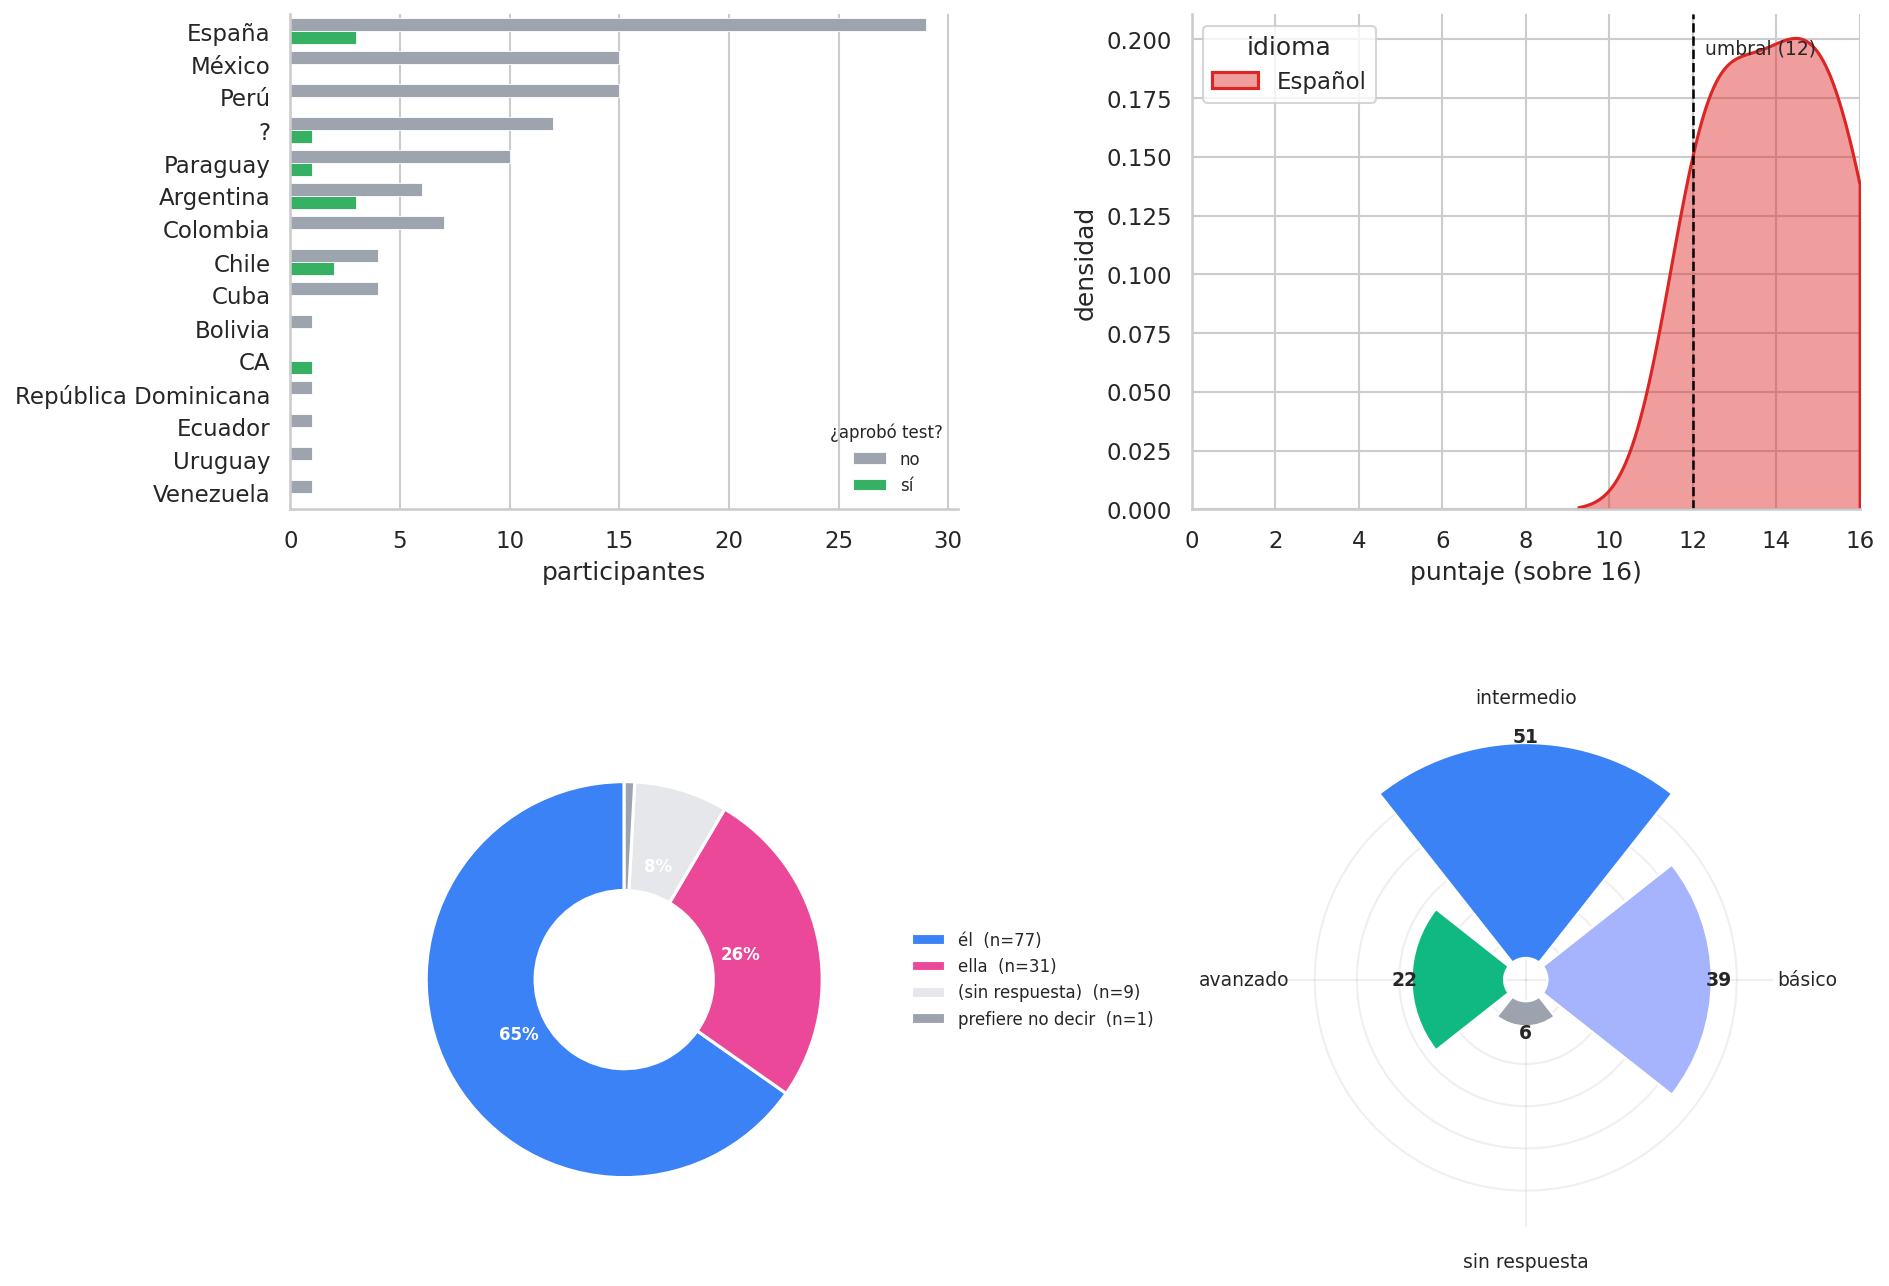
\includegraphics[width=0.95\textwidth]{panorama_demografico.png}
    \caption{Panorama demográfico de los 118 participantes registrados. Panel superior izquierdo: distribución por país, con barras coloreadas según si el participante aprobó el test de entrada (verde = sí, gris = no). Panel superior derecho: estimación de densidad de los puntajes del test, segmentada por idioma de la interfaz; la línea discontinua marca el umbral de aprobación de 12 sobre 16. Panel inferior izquierdo: distribución de pronombres como gráfico de dona. Panel inferior derecho: barras polares con el nivel autodeclarado de conocimiento de PLN.}
    \label{fig:panorama_demografico}
\end{figure}
